\section{Introduction}
Here interaction quench in paramagetic Hubbard model(HM) is studied using non equilibrium DMFT IPT developed by Naoto Tsuji. This code is attached as supplementary material of 2014 RMP paper\cite{RMP}. I have tried to reproduce the published results in PRL \cite{HUB_para} paper 2009 and \cite{HUB} in 2013.

In the public version of code they have implemented bare 2 nd order perturbation theory with Kadanoff-Baym formalism.

%Their study shows that for large interaction  bare 4 th order perturbation theory give qualitative same result as QMC.

%I have been thinking i can study the IHM paramagnetic case $\delta$ quenching for small U with this 2 nd order perturbation theory code.


\section{double occupancy(d) and jump in distribution function($\Delta n$)  }

\begin{figure}[H]
%\centering
\begin{subfigure}{.5\textwidth}
 % \centering
 \includegraphics[width=1.\linewidth]{bench_marking/HUB_para_quench_literature_small_U.png}
  \caption{}
  %\label{fig:sub1}
\end{subfigure}%
\begin{subfigure}{.5\textwidth}
 % \centering
  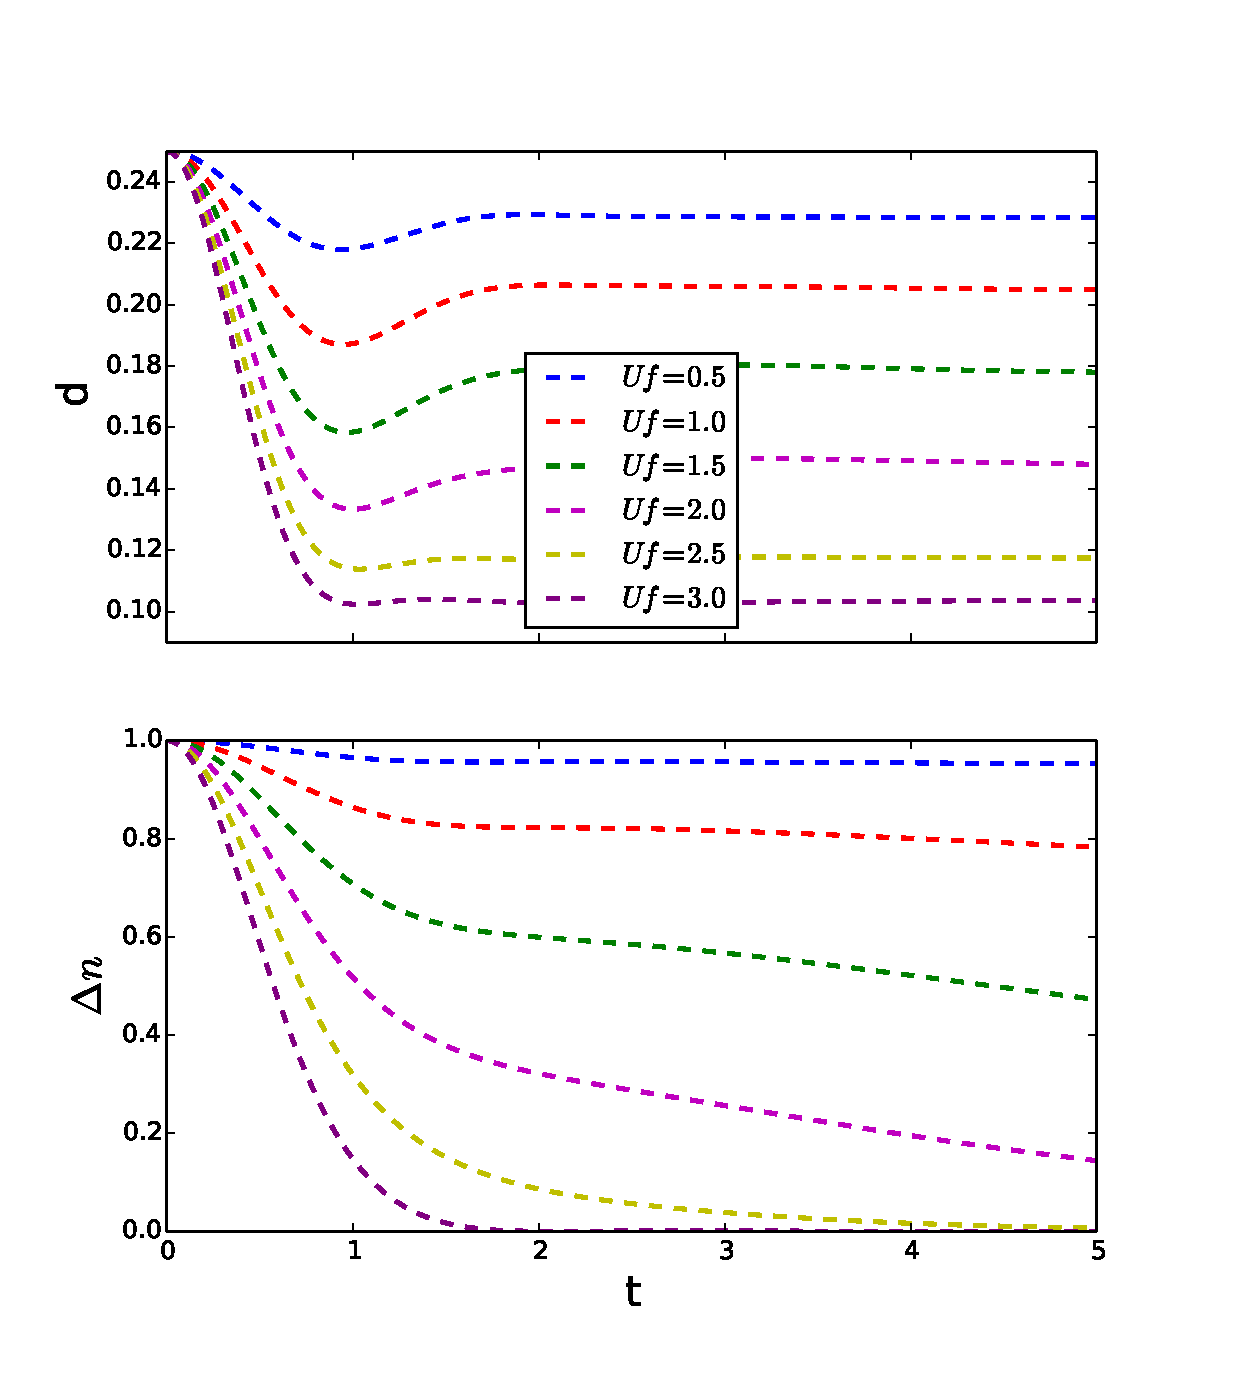
\includegraphics[width=1.\linewidth]{bench_marking/dn_d.eps}
  \caption{parameters are same as figure (a). d and $\Delta n$ calculated using second order bare IPT. main code is written by Naoto Tsuji and attached to RMP\cite{RMP}. $\Delta n$ measurement part is added later with original code by Soumen Bag   }
  %\label{fig:sub2}
\end{subfigure}
\caption{}
\label{d_dn}
\end{figure}

In figure \ref{d_dn}.(b) double occupancy(d) and jump of the momentum distribution function($\Delta n$) calculated using bare second order IPT code is written by Naoto Tsuji and attached to RMP\cite{RMP} compared with dashed line in \ref{d_dn}.(a) calcuted using bold second order IPT taken from \cite{HUB}. one notice that bare second order IPT underestimat both d and $\Delta n$ compare with bold second order IPT.


\begin{figure}[H]
%\centering
\begin{subfigure}{.5\textwidth}
 % \centering
 \includegraphics[width=1.1\linewidth]{bench_marking/HUB_para_quench_literature_large_U.png}
  \caption{}
  %\label{fig:sub1}
\end{subfigure}%
\begin{subfigure}{.5\textwidth}
 % \centering
  \includegraphics[width=1.1\linewidth]{bench_marking/HUB_para_quench_code_large_U.pdf}
  \caption{}
  %\label{fig:sub2}
\end{subfigure}
%\caption{dos for $\Delta=1.0t$, $t_2 = 0.4t$(a) at U = 0.4t band insulator  (b) at U = 2.0t metal}
%\label{fig:test}
\end{figure}
%###############################################################################################3
\section{Total energy}
\begin{figure}[H]
%\centering
\begin{subfigure}{.5\textwidth}
 % \centering
 \includegraphics[width=1\linewidth]{bench_marking/energy_lit.png}
  \caption{symbol for CTQMC, dashed line are IPT, solid line are SPT(self-consistent perturbation theoty) is taken from \cite{HUB1}}
  %\label{fig:sub1}
\end{subfigure}%
\begin{subfigure}{.5\textwidth}
 % \centering
  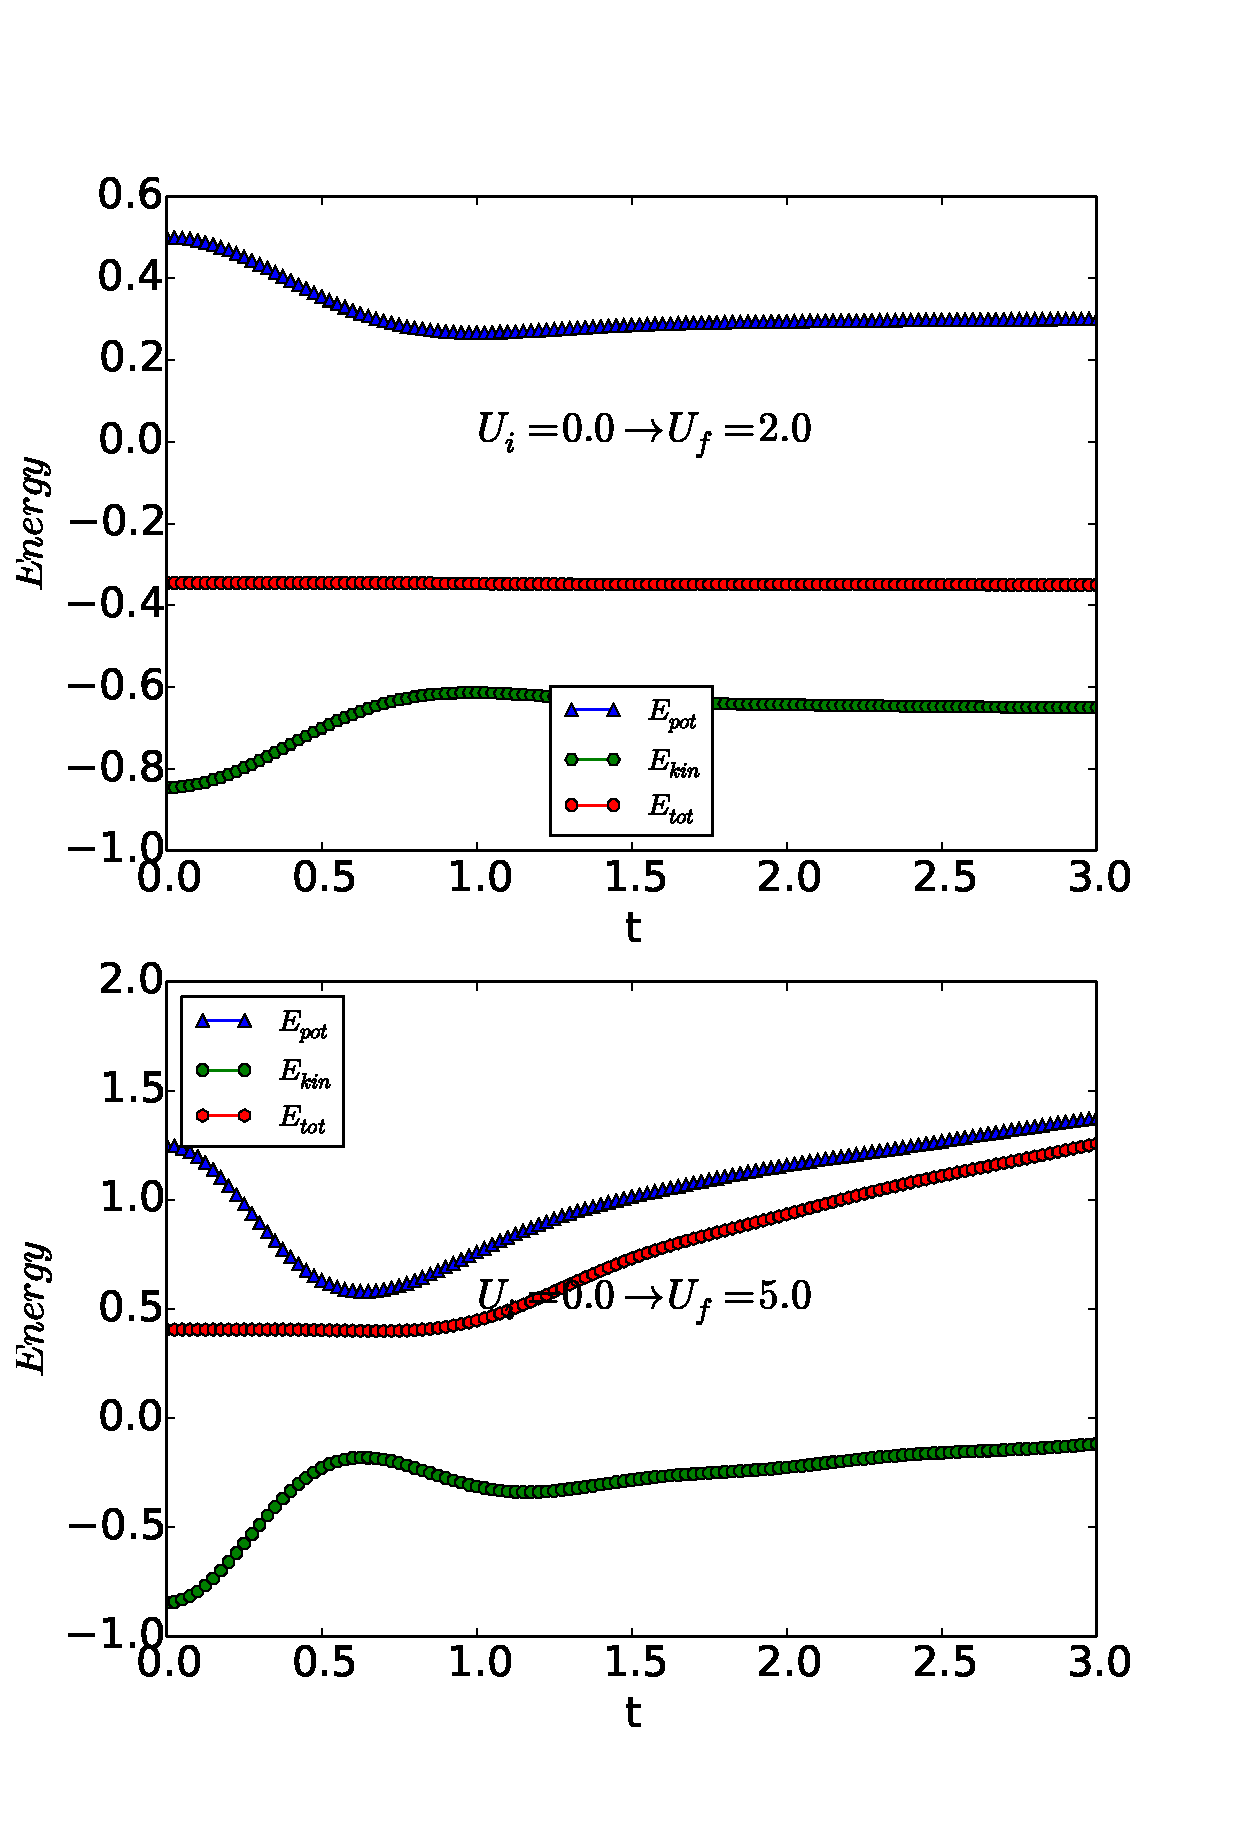
\includegraphics[width=1\linewidth]{bench_marking/energy.eps}
  \caption{2 nd order bare IPT}
  %\label{fig:sub2}
\end{subfigure}
\caption{}
%\label{fig:test}
\end{figure}

For $U_f$ > 3.3 we see the 2 nd order IPT does not conserve the energy. it has been observed that if one do more accurate calculation like ctqmc \cite{HUB} energy remain converse which is expected.
%############################################################
\section{effective temparature}
\begin{figure}[H]
%\centering
\begin{subfigure}{.5\textwidth}
 % \centering
 \includegraphics[width=1.1\linewidth]{bench_marking/total_energy_vs_beta_U1.eps}
  \caption{sustem is quenched form U = 0.0  at $\beta$ = 16 or T=0.0625 to U=1.0t. then effective temperature(T*) of the system is crossing point. T*=0.15 }
  %\label{fig:sub1}
\end{subfigure}%
\begin{subfigure}{.5\textwidth}
 % \centering
  \includegraphics[width=1.1\linewidth]{bench_marking/total_energy_vs_beta_U2.eps}
  \caption{effective temperature(T*)=0.28}
  %\label{fig:sub2}
\end{subfigure}
%\caption{dos for $\Delta=1.0t$, $t_2 = 0.4t$(a) at U = 0.4t band insulator  (b) at U = 2.0t metal}
%\label{fig:test}
\end{figure}

total energy of the HM at U=1.0, 2.0 is plotted as a function of beta($\beta$). Horizontal line correspond the energy after interaction quench. Intersection point is the temperature  of the system after interaction quench. 

\begin{figure}[H]
%\centering
\begin{subfigure}{.5\textwidth}
 % \centering
 \includegraphics[width=1.1\linewidth]{bench_marking/total_energy_vs_beta_U3.eps}
  \caption{effective temprature(T*) = 0.70}
  %\label{fig:sub1}
\end{subfigure}%
\begin{subfigure}{.5\textwidth}
 % \centering
  \includegraphics[width=1.1\linewidth]{bench_marking/total_energy_vs_beta_U33.eps}
  \caption{effective temprature(T*) = 0.90}
  %\label{fig:sub2}
\end{subfigure}
%\caption{dos for $\Delta=1.0t$, $t_2 = 0.4t$(a) at U = 0.4t band insulator  (b) at U = 2.0t metal}
%\label{fig:test}
\end{figure}

we see the interaction is quenched with initial non-interating state at T=0.0625. effective temperature of the system increases with the quenched interaction value.
